\section{Software project management}
\subsection{What is Software Project Management}
Software project management ist essenziell um
\begin{itemize}
	\item Software pünktlich zu liefern
	\item Kosten im Budget zu halten
	\item Software zu liefern, die die Erwartungen der Kunden erfüllen
	\item ein gut funktionierendes Entwicklungsteam zu erhalten
\end{itemize}
\subsubsection{Important factors}
\begin{itemize}
	\item Firmengröße
	\item Software-Kunden
	\item Softwaregröße
	\item Organisationskultur
	\item Software development processes
\end{itemize}
\subsubsection{Main activities}
\begin{itemize}
	\item Projektplanung
	\item Risikomanagement
	\item People-Management
	\item Meldung
	\item Vorschlägeschreiben
\end{itemize}
\subsubsection{Project management triangle}
\begin{table}[H]
\caption{Project management triangle}
\begin{center}
	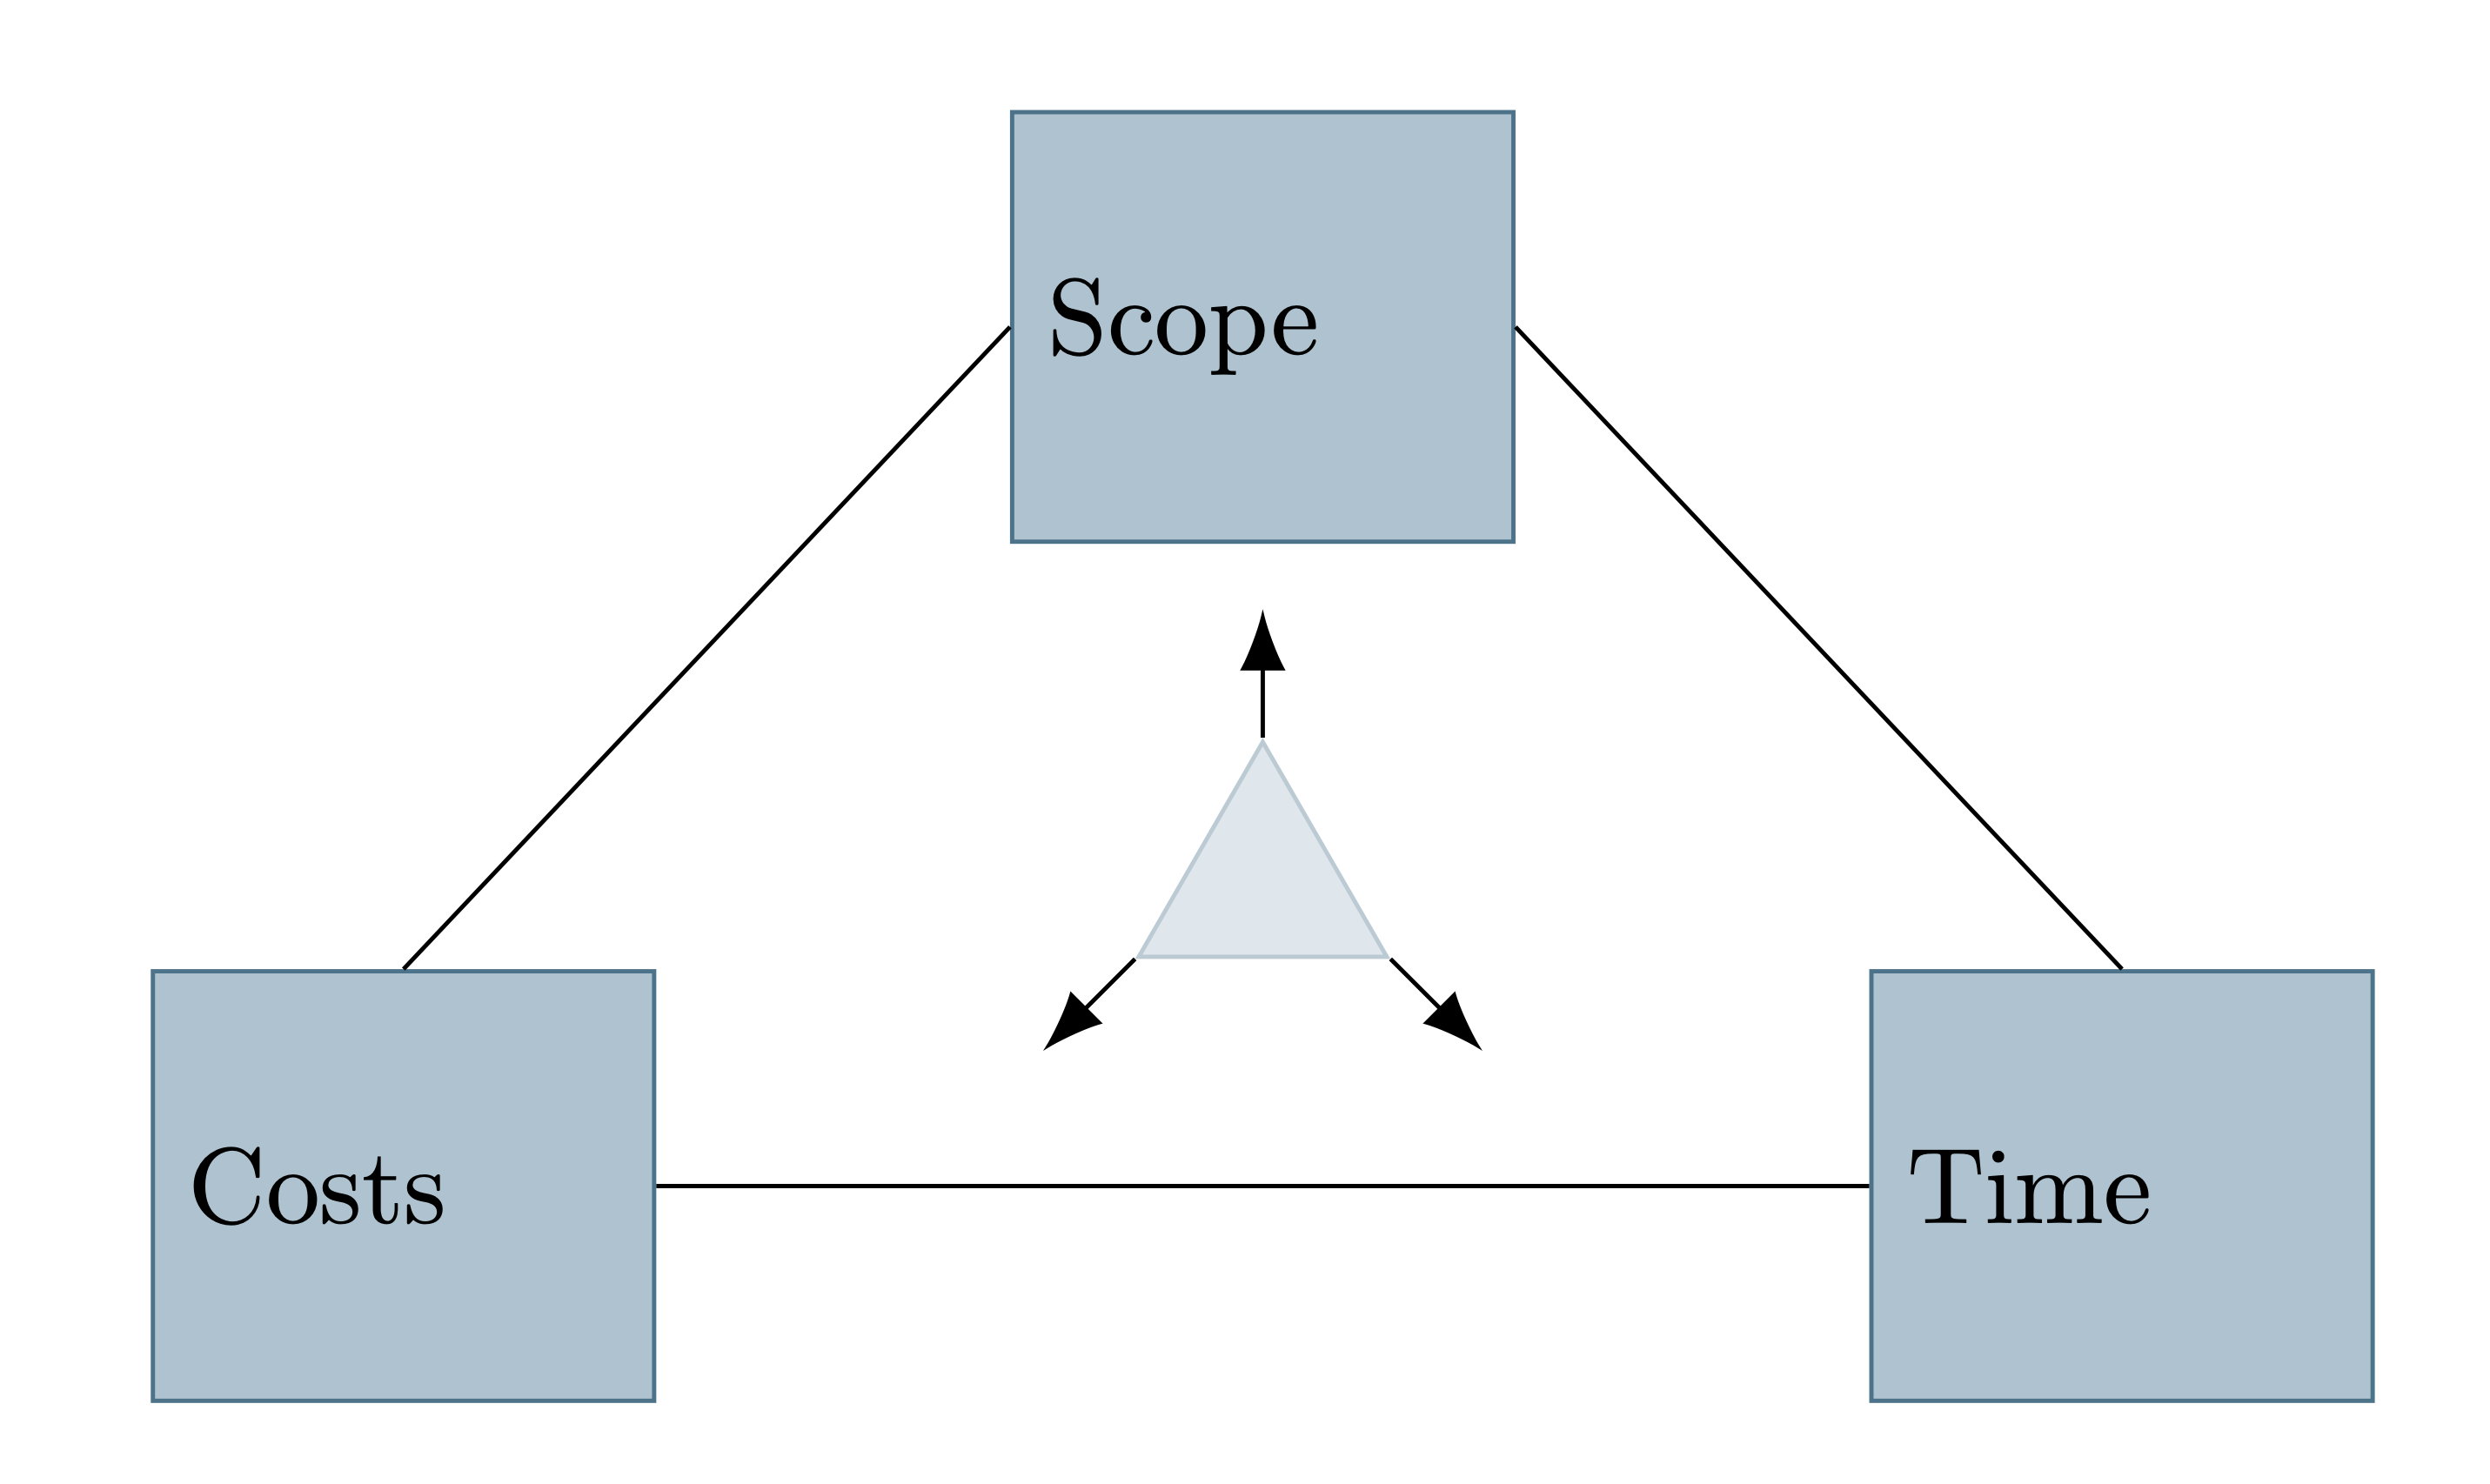
\includegraphics[scale=0.25]{Project_,management_triangle.png}
\end{center}	
\end{table}
Änderung einer Einschränkung verändert die Werte der anderen 
\subsubsection{Five smart criteria}
\begin{itemize}
	\item Spezifisch
	\item Messbar 
	\item Assignable 
	\item Realistisch
	\item Zeitabhängig
\end{itemize}
\subsection{Time management}
\subsubsection{Project scheduling}
\begin{itemize}
	\item Wie wird die Arbeit in separate Aufgaben aufgeteilt
	\item Wann und wie werden diese Aufgaben bearbeitet
	\item Wer die Aufgaben zugeschrieben bekommt
	\item Wie viel Zeit ist nötig um eine Aufgabe zu erledigen
	\item Welche Hardware- und Softwareresourcen werden benötigt
\end{itemize}
\subsubsection{Activity-on-arrow diagram}
\begin{table}[H]
\caption{AoA diagram}
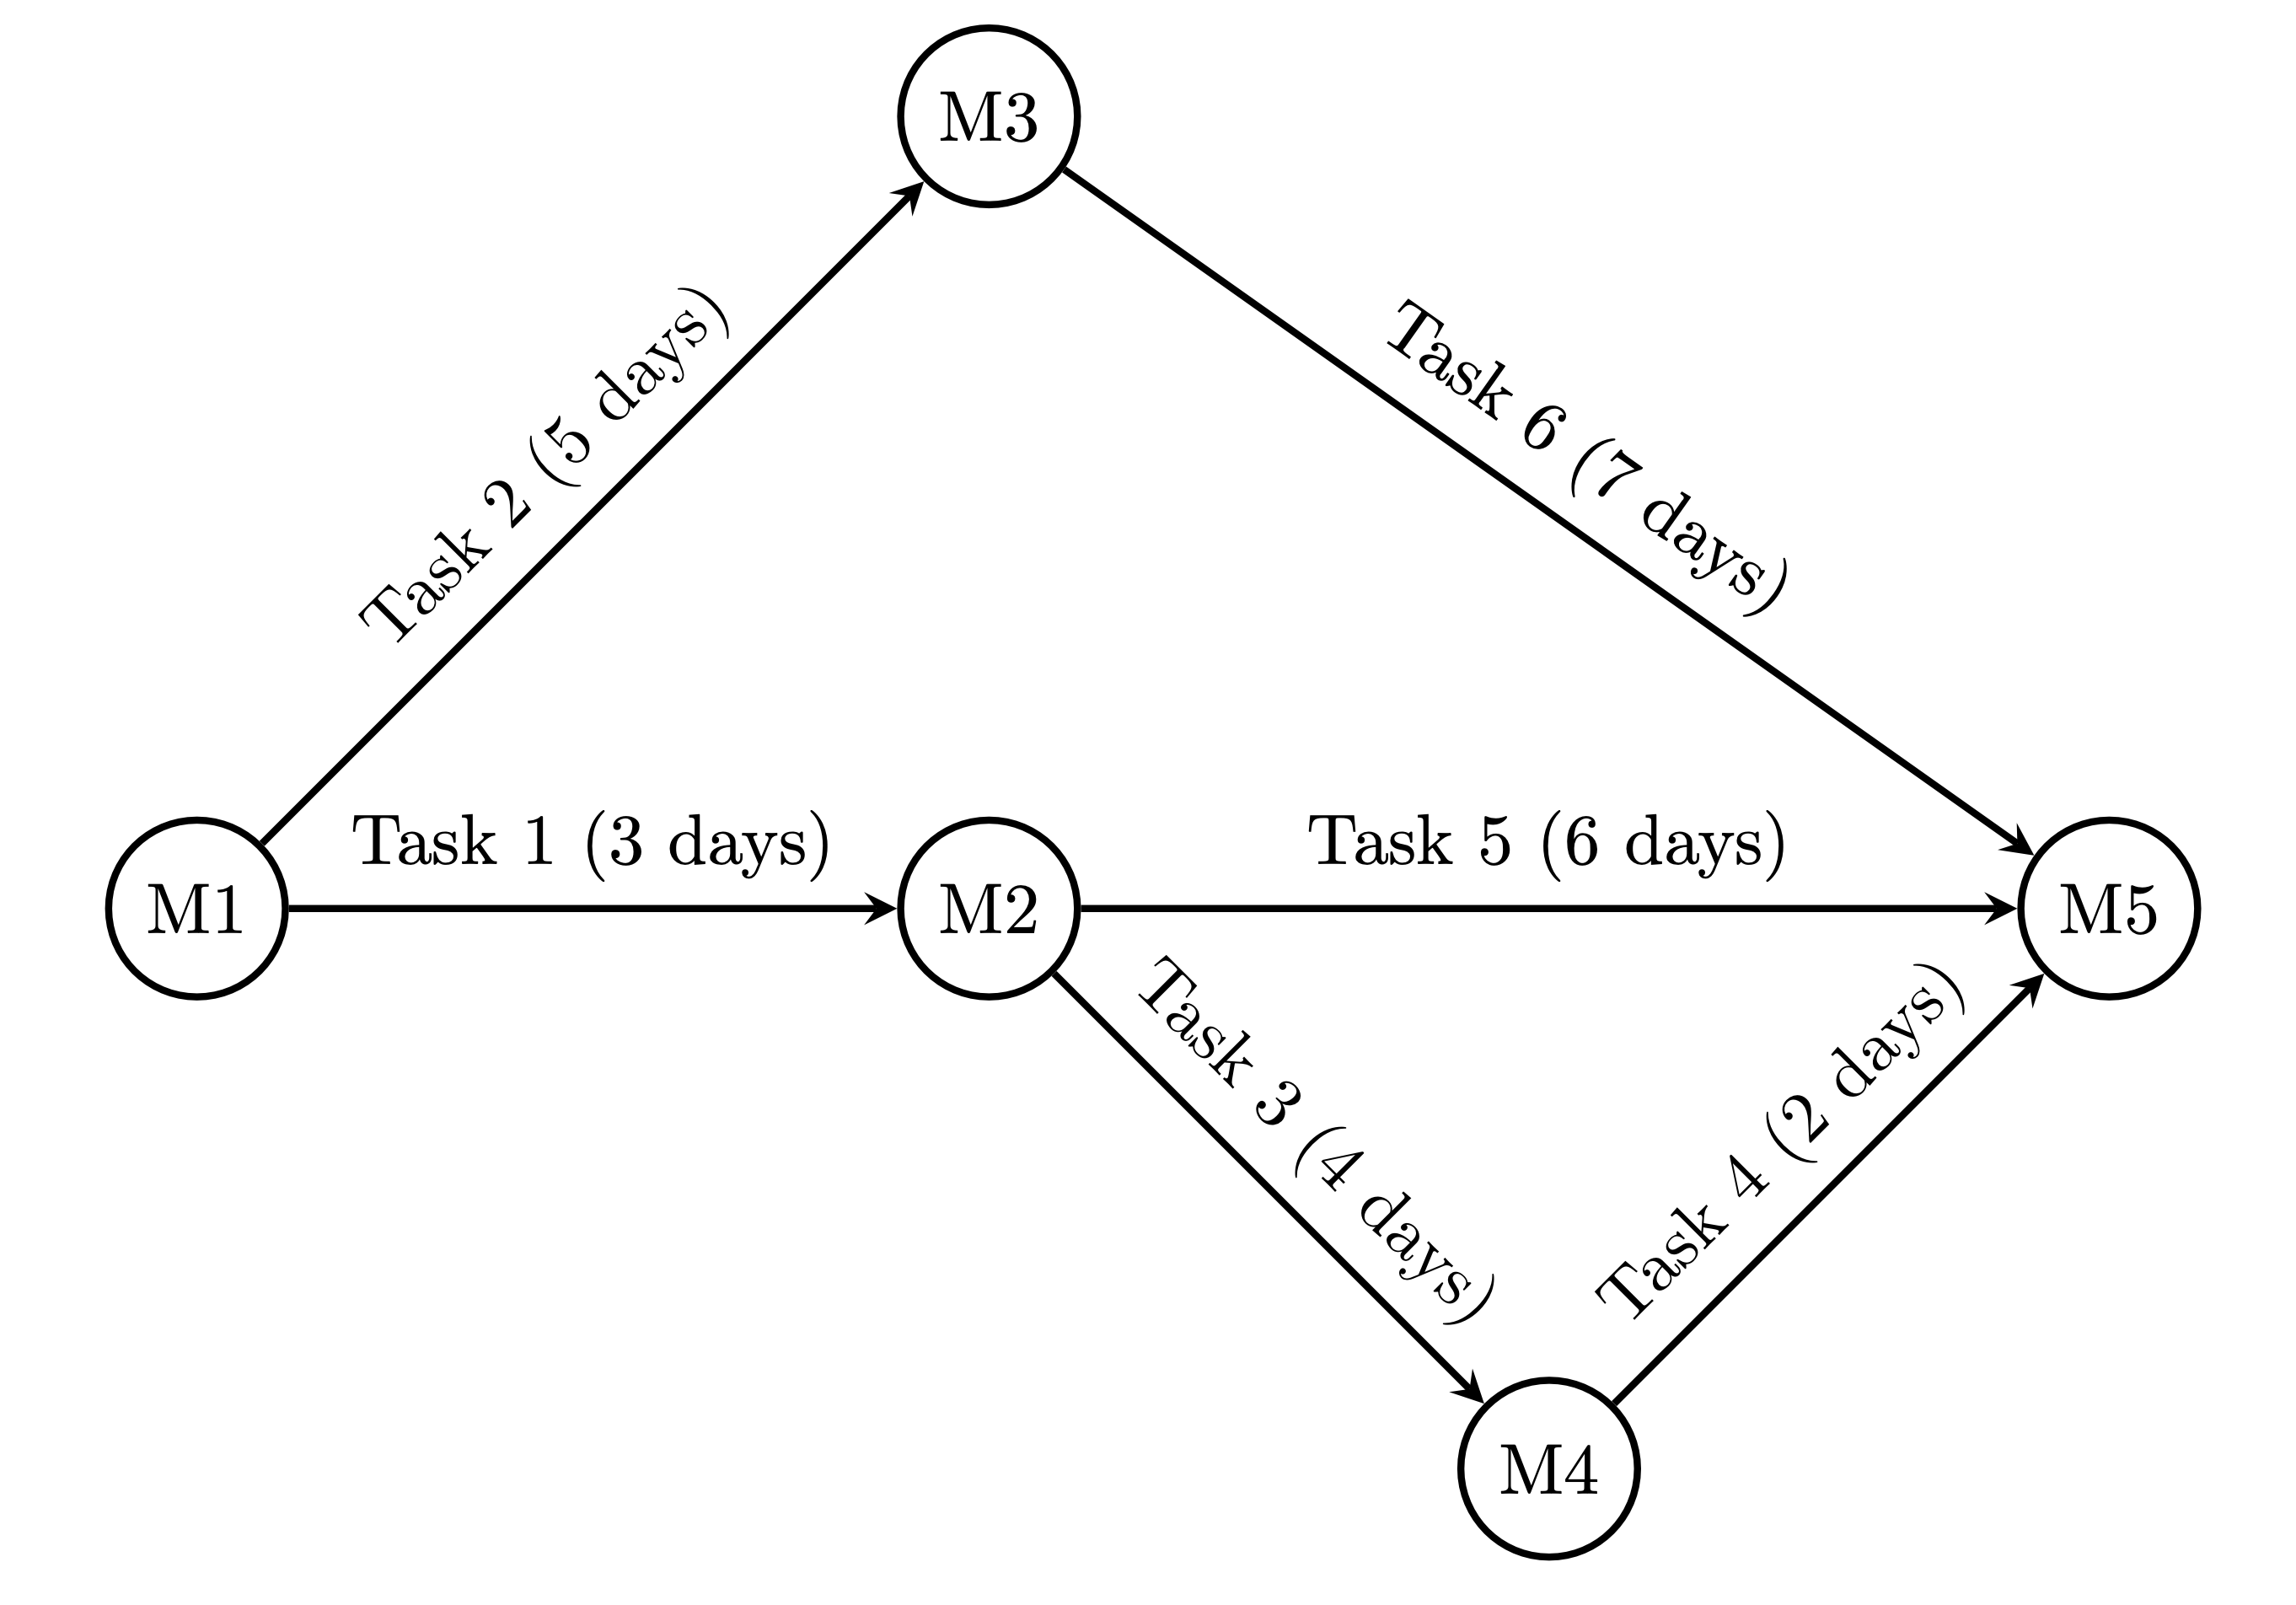
\includegraphics[scale=0.25]{AOA_diagram.png}
\end{table}
\begin{itemize}
	\item Knoten: Milestones
	\item Pfeile: Aktivitäten
\end{itemize}
\subsubsection{Activity-on-node diagram}
\begin{table}[H]
\caption{AoN diagram}
\begin{center}
	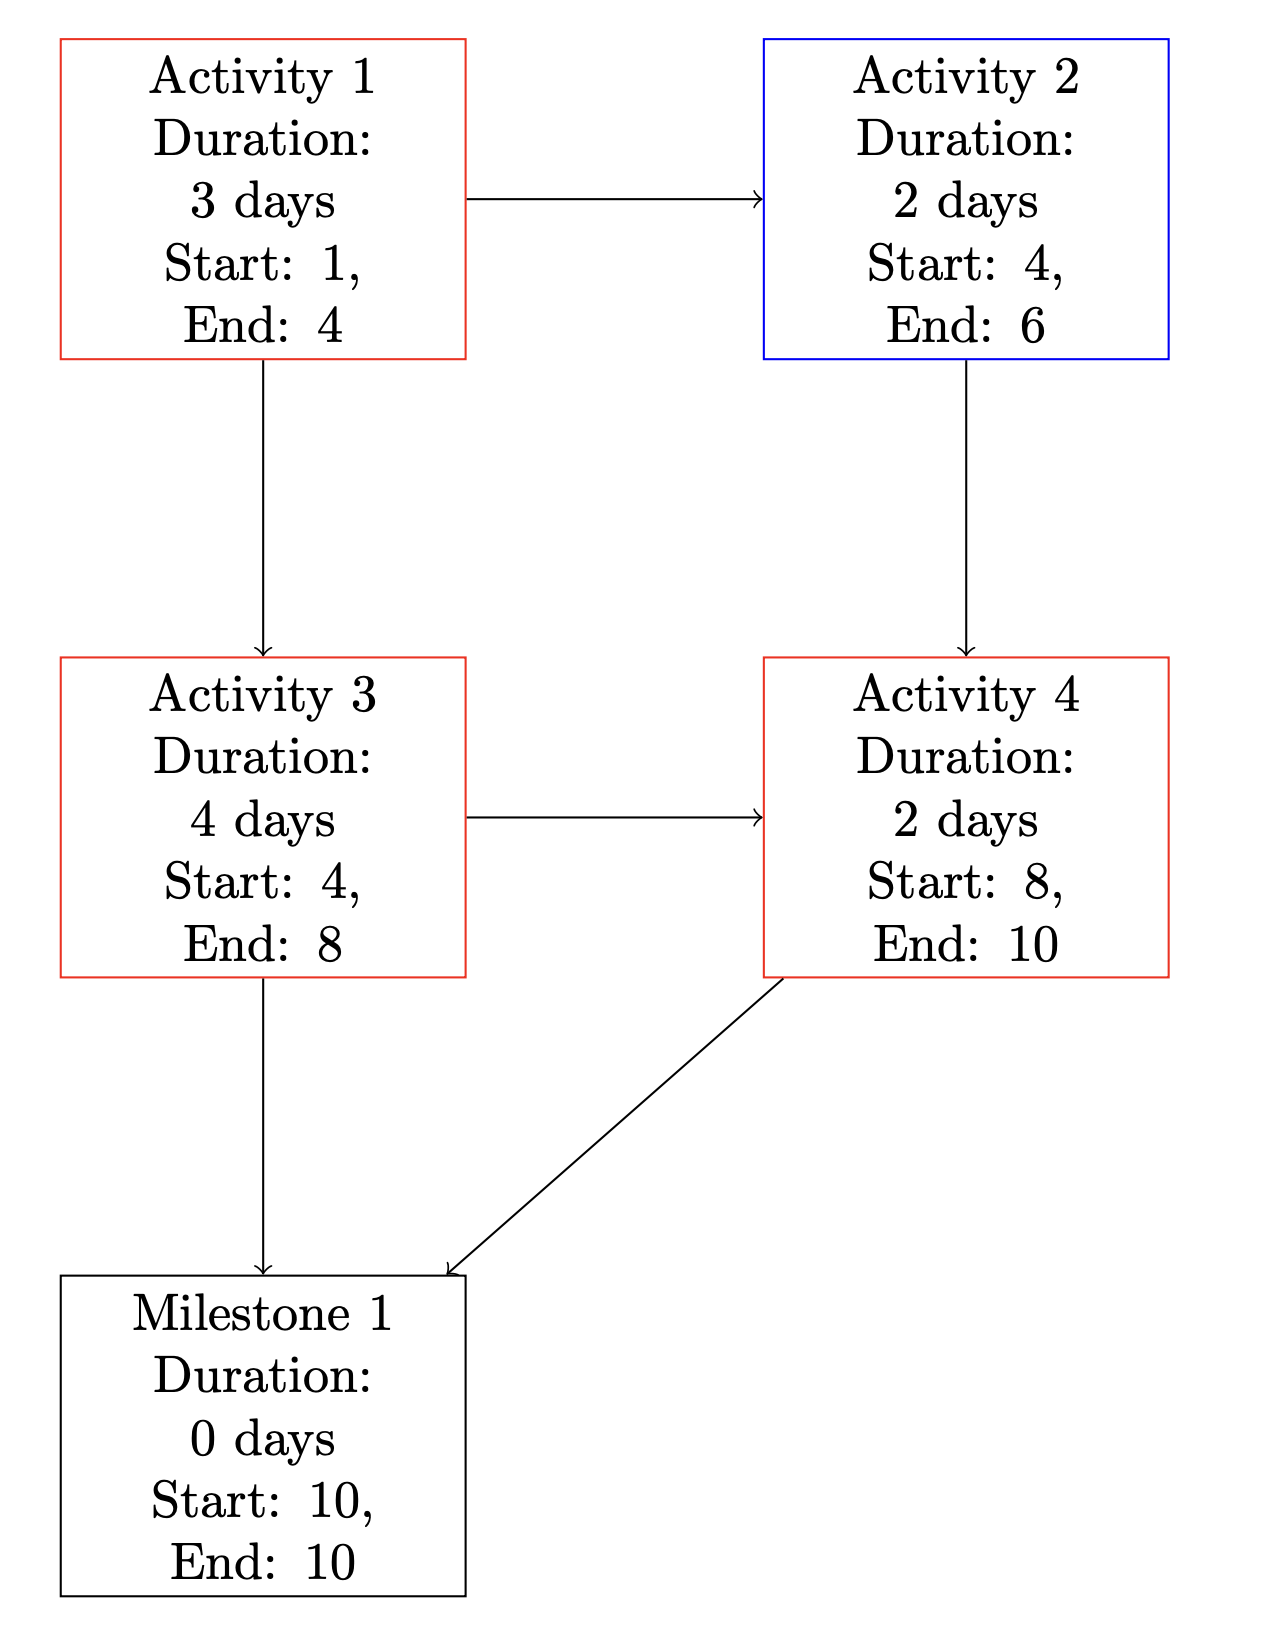
\includegraphics[scale=0.25]{AON_diagram.png}
	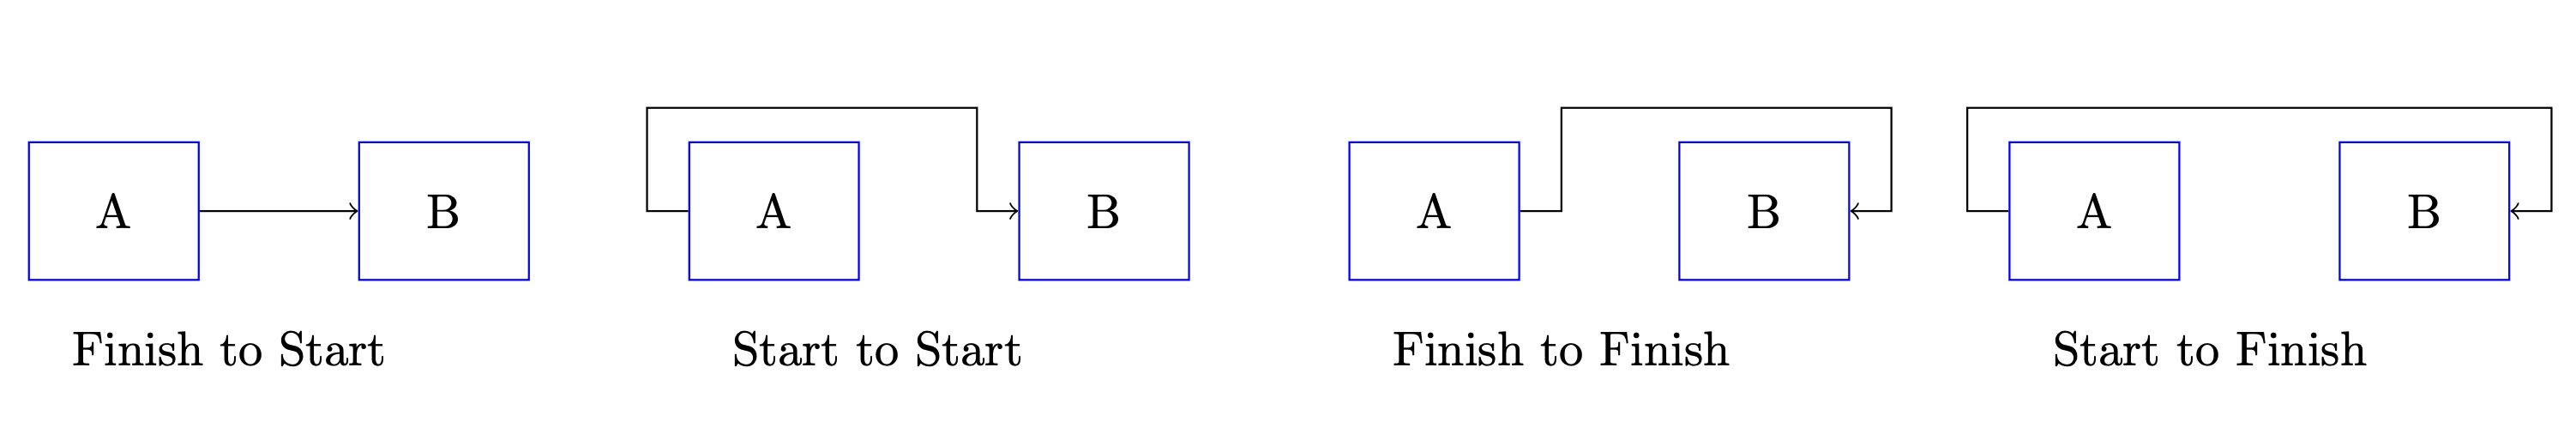
\includegraphics[scale=0.25]{AON_relations.png}
\end{center}
\end{table}
\begin{itemize}
	\item F $\to$ S: B kann erst beginnen, wenn A fertig ist
	\item S $\to$ S: B kann erst beginnen, wenn A begonnen hat
	\item F $\to$ F: B kann erst enden, wenn A beendet ist
	\item S $\to$ F: B kann erst enden, wenn A begonnen hat
\end{itemize}
Die benötigte Zeit für einen Durchlauf kann anhand des kritischen Pfades + die Zeit für alle Aufgaben berechnet werden 
\subsubsection{Gnatt chart}
\begin{table}[H]
\caption{Gantt chart}
\begin{center}
	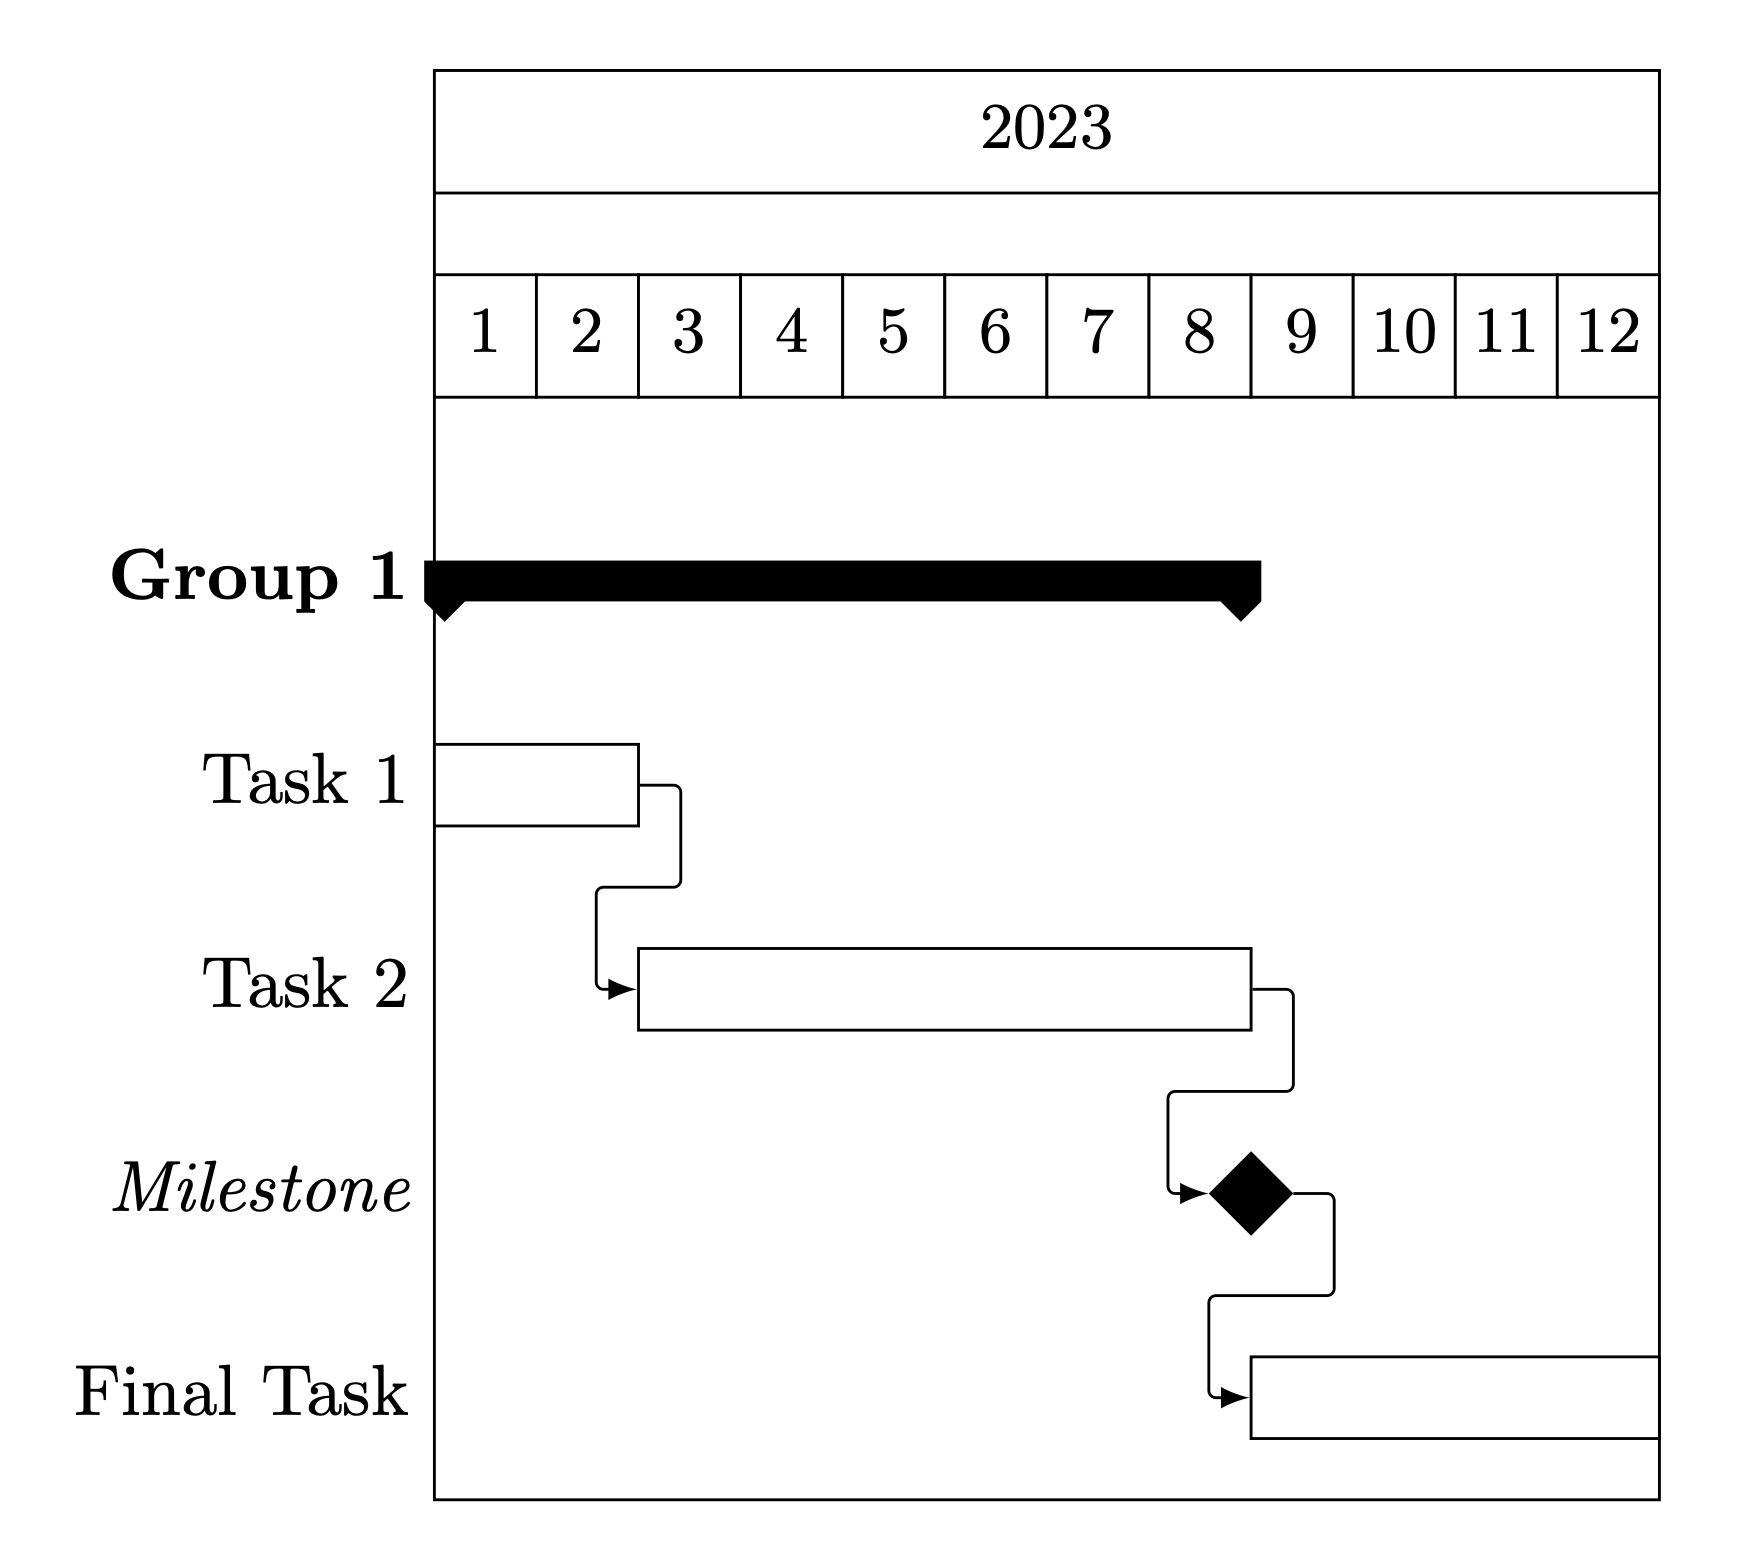
\includegraphics[scale=0.25]{Gnatt.png}
\end{center}	
\end{table}
\subsection{Cost Management}






